\documentclass{elsarticle}
\usepackage{graphicx}
%\usepackage{multicol}
%\usepackage{footmisc}
\usepackage{amstext}
\usepackage{amsmath}
\usepackage{amssymb}
\usepackage{amsthm}
\usepackage[english]{babel}
%\usepackage[official,right]{eurosym}
\selectlanguage{english}
\hyphenation{ExecEngine}
\newtheorem{lemma}{Lemma}
\def\Events{{\mathit E}}
\begin{document}
% Ampersand -----------------------------------------------------------

%\def\id#1{\text{\it #1\/}}
\newcommand{\id}[1]{\text{\it #1\/}}
\newcommand{\code}[1]{\text{\tt\small #1}}
\newcommand{\stmtText}[1]{``{\small\tt #1}''}
\newcommand{\dom}[1]{\id{dom}(#1)}
\newcommand{\cod}[1]{\id{cod}(#1)}
\renewcommand{\int}[2]{\id{inter}(#1,#2)}
\newcommand{\relsIn}[1]{\id{relsIn}(#1)}    % maps a Term to a set of Relations
\newcommand{\maintain}{\id{maint}}
\newcommand{\pop}[2]{\id{pop}_{#1}(#2)}
\newcommand{\inst}{\id{inst}}
\newcommand{\relname}[1]{\id{relname}(#1)}
\newcommand{\src}[1]{\id{src}(#1)}
\newcommand{\tgt}[1]{\id{tgt}(#1)}
\newcommand{\sat}[2]{\id{sat}_{#1}(#2)}
\newcommand{\viol}[2]{\id{viol}_{#1}(#2)}
\newcommand{\sign}[1]{\id{sign}(#1)}
\newcommand{\powerset}[1]{\cal{P}\{#1\}}
\newcommand{\theCode}{\url{http://cs.ru.nl/~B.Joosten/ampTypes/}}
\newcommand{\la}{\langle}
\newcommand{\ra}{\rangle}
\newcommand{\full}{V}
\newcommand{\declare}[3]{\id{#1}_{\pair{#2}{#3}}}
\newcommand{\subst}[3]{#3_{[#1\rightarrow #2]}}
\newcommand{\fullt}[2]{V_{\pair{#1}{#2}}}
\newcommand{\iden}{I}
\newcommand{\ident}[1]{I_{\id{#1}}}
\newcommand{\expr}[3]{(#1)_{#2\times #3}}
\newcommand{\pair}[2]{\la{#1},{#2}\ra}
\newcommand{\Pair}[2]{#1\times#2}
\newcommand{\pairs}[1]{\id{pairs}(#1)}
\newcommand{\triple}[3]{\la{#1},{#2},{#3}\ra}
\newcommand{\quadruple}[4]{\la{#1},{#2},{#3},{#4}\ra}
\newcommand{\atom}[1]{{\tt\small #1}}
\newcommand{\atoms}{\mathcal{A}}
\newcommand{\Atoms}{\mathbb{A}}
\newcommand{\concept}[1]{{\tt\small #1}}
\newcommand{\concepts}{\mathcal{C}}
\newcommand{\Concepts}{\mathbb{C}}
\newcommand{\decls}{\mathcal{D}}  %% names of relations
\newcommand{\rels}{\mathcal{R}}   %% all relations
\newcommand{\Rels}{\mathbb{R}}   %% all relations
\newcommand{\relations}{\mathcal{M}} % representing terms. M is a subset of R.
\newcommand{\triples}{\mathcal{T}}
\newcommand{\Triples}{\mathbb{T}}
\newcommand{\Triple}[3]{#1\times#2\times#3}
\newcommand{\vertices}{N}
\newcommand{\rules}{\mathcal{U}}
\newcommand{\Rules}{\mathbb{U}}
\newcommand{\specrules}{\mathcal{S}}
\newcommand{\roles}{\mathcal{O}}
\newcommand{\Events}{{\mathit E}}
\newcommand{\dataset}{\mathscr{D}}
\newcommand{\Dataset}{\mathbb{D}}
\newcommand{\schema}{\mathscr{Z}}
\newcommand{\functionality}{\mathscr{F}}
\newcommand{\select}[2]{\id{select}_{#1}\{{#2}\}}
\newcommand{\migrsys}{\mathscr{M}}
\newcommand{\infsys}{\mathscr{S}}
\newcommand{\tf}[1]{\mathscr{T}(#1)}
\newcommand{\ptf}[1]{\mathscr{T}'(#1)}
\newcommand{\ti}[1]{\mathscr{I}(#1)}
\newcommand{\tic}[1]{I_{\cal C}(#1)}
\newcommand{\relAdd}{\dagger}
\newcommand{\flip}[1]{{#1}^\smallsmile} %formerly:  {#1}^\backsim
\newcommand{\kleeneplus}[1]{{#1}^+}
\newcommand{\kleenestar}[1]{{#1}^*}
\newcommand{\cmpl}[1]{\overline{#1}}
\newcommand{\rel}{\times}
\newcommand{\compose}{;}
\newcommand{\subs}{\subseteq}%{\models}
\newcommand{\fun}{\rightarrow}
\newcommand{\isa}{\preceq}
%\newcommand{\isaClos}{\sqsubseteq}
\newcommand{\typetest}{?}
\newcommand{\meet}{\sqcap}
\newcommand{\join}{\sqcup}
\newcommand{\Meet}{\bigsqcap}
\newcommand{\Moin}{\bigsqcup} % because LaTeX has already defined command \Join.
\newcommand{\order}{\ominus}
\newcommand{\anything}{\top}
\newcommand{\nothing}{\bot}
\newcommand{\rewriteto}{\rightarrow}
\newcommand{\calc}{\implies}
\newcommand{\alland}{\bigwedge}
\newcommand{\mph}[3]{#1_{#2\times #3}}
\newcommand{\mphu}[1]{#1_{\univ\times\univ}}

%-----------------------------------------
\newcommand{\kse}{\hspace*{1.7em}}
\newcommand{\ksf}{\hspace*{1em}}
\newcommand{\ksg}{\hspace*{1em}}
\newenvironment{derivation}{\begin{tabbing}\kse \= \ksf \= \ksg \= \kill}{\end{tabbing}}
\newtheorem{definition}{Definition}
\newcommand{\term}[1]{\>\>\(#1\)\\[1ex]}
\newcommand{\rela}[2]{\>\(#1\)\>\>\{ \ #2 \ \}\\[1ex]}
\newcommand{\weg}[1]{}

\def\define#1{\label{dfn:#1}{\em #1}\index{#1}}
\def\definem#1{\label{dfn:#1}{\em #1}\index{#1}\marge{#1}}
\newcommand{\marg}[1]{\index{#1}\marge{#1}}


\title{A Theory for Migration of Information Systems}
\author[ou,ordina]{Stef Joosten\fnref{fn1}}
\ead{stef.joosten@ou.nl}
\author[umn]{Sebastiaan Joosten\fnref{fn2}}
\address[ou]{Open Universiteit Nederland, Heerlen, the Netherlands}
\address[ordina]{Ordina NV, Nieuwegein, the Netherlands}
\address[umn]{University of Minnesota, Minneapolis, USA}
\fntext[fn1]{ORCID 0000-0001-8308-0189}
\fntext[fn2]{ORCID 0000-0002-6590-6220}

\begin{abstract}
	The Ampersand project has provided the theory and tools to generate semantic information systems from an algebraic specification.
	However, information systems in practice may change repeatedly after their maiden deployment.
	Changes that affect the data model typically result in a data migration.
	In such cases, simply regenerating the system is not enough because it would reset the database to its initial state (deleting all data gathered so far).
	Migration aims at preserving the data as much as possible.
	Typically, migration involves transferring the old data to the new system while preserving the semantics as much as possible.

	In this contribution we develop a theory for reliable data migration that aims at automating it as much as possible,
	to enable more frequent migrations.
	The ultimate target is to generate a migration from two specifications: the as-is specification and the to-be specification.
	A software generator that embodies this theory is subject of future research.
\end{abstract}

\begin{keyword}
relation algebra\sep software development\sep data migration\sep software migration\sep Ampersand
\end{keyword}
\maketitle

\section{Introduction}
\label{sct:Introduction}
	The challenge of migration is to preserve meaning rather than just copy the data from one place to another.

\section{Migration steps}
	A smooth migration from an old system to a new system would go as follows:
	Launch the new system in parallel to the old, copy data from the old to the new system, and have everyone use the new system.
	We identify the following possible issues in this approach:

	\begin{enumerate}
	\item Data required in the new system is missing in the old system.
	There may be no way in the old system to enter that data.
	An example could be that every reimbursement form needs to have an address associated to it to mail the check to, but address information is not stored in the old system:
	The old system required the reimbursement office to look up employee's addresses from a hand-written list they had on their desk.
	\item Data in the old system is wrong but cannot be corrected there due to how the old system was designed.
	An example is if the old system only allows approvals to be entered as the current user, and the CEO insists that her administrative staff enters his approvals into the system for her.
	This may result in approvals being entered as admin staff, where it was really the CEO making the approval.
	\item Data in the old system does not satisfy invariants of the new system.
	There may be no way in the old system of making the data satisfy those invariants. We can use the same example as in the previous bullet point, but add the requirement (in the new system) that every purchase above a certain amount needs to be approved by the CEO.
	\item A way of entering data into the old system is missing in the new system.
	People or automated processes might rely on these ways of entering data.
	An example could be that when employees turned their computers on or off, an ad-hoc script would automatically clock them in- and out to determine the number of hours they worked.
	A handful of employees still relies on this.
	\item Data present in the old system cannot be stored in the new system.
	An example could be that references to physical locations where original receipts are kept are stored in the old system, but the new system relies on scans of receipts and allows the originals to be destroyed or not submitted.
	Until the original receipts are scanned, the old data should be kept.
	\end{enumerate}
	
	To mitigate these issues, we:
	
	\begin{enumerate}
	\item Allow `missing' triples requirements to be ignored during migration.
	\item Allow triples to be migrated while being marked as needing correction.
	\item Allow invariants in the new system to be ignored for certain triples during migration.
	\item Allow continued use of interfaces of the old system, data entered into the old system via those interfaces needs to be continuously copied to the new system.
	\item Retain data in the old system until it can be marked as ready to be phased out.
	\end{enumerate}	

\section{Terminology}
\label{sct:Terminology}
	Migration is sometimes called data migration, because most people understand that data from "the old system" is fed into "the new system".
	The idea is that the new system lets the business continu without interruption, after its software has been upgraded.
	Since data is so central to migration, we start by introducing the notion of dataset.
	To abstract away from a particular database implementation,
	we represent data elements as triples.
	This makes our theory valid for any kind of database that triples can represent,
	such as SQL databases, object-oriented databases, graph databases, triple stores, and other no-SQL databases

	Migration is not just about porting data.
	It is about preserving the meaning of that data.
	For that purpose, section~\ref{sct:Information Systems} introduces the notion of information system.

\subsection{Datasets}
	A dataset describes a set of structured data, which is typically stored persistently in a database of some kind.

	Before defining datasets, we must first define the constituent notions of atom, concept, triple, and relation.
	
	Atoms serve as data elements.
	They are values without internal structure of interest, meant to represent data elements in a database.
	From a business perspective, atoms are used to represent concrete items of the world,
	such as \atom{Peter}, \atom{1}, or \atom{the king of France}.
	By convention throughout the remainder of this paper, variables $a$, $b$, and $c$ are used to represent \emph{atoms}.
	The set of atoms is called $\atoms$.
	

	Concepts are names we use in a conceptual model during the design of a dataset.
	They are also used to assign signatures to relations, to enable type checking on the dataset.
	For example, you might choose to classify \atom{Peter} as a \concept{Person}, and \atom{074238991} as a \concept{TelephoneNumber}.
	In this example, \concept{Person} and \concept{TelephoneNumber} are concepts.
    We will use variables $A$, $B$, $C$, $D$ to represent concepts.
	The term $\ident{A}$ represents the \emph{identity relation} of concept $A$.
	The expression $a\ \inst\ A$ means that atom $a$ is an \emph{instance} of concept $A$.
	The statement $A\isa B$ (pronounce: $A$ is a $B$) states that any instance of $A$ is an instance of $B$ as well.
	We call this {\em specialization}, but it is also known as {\em generalization} or {\em subtyping}.
	Specialization is needed to allow statements such as: ``A woman is a human'' or ``A human is a mammal''.
	The set of concepts is called $\concepts$.
	
	Triples are used to represent data.
	Each triple relates two atoms to a relation.
	A triple $\triple{\text{\atom{Peter}}}{\id{phone}}{\text{\atom{074238991}}}$ might mean that the ``thing'' that \atom{Peter} refers to
	has \atom{074238991} as a telephone number.
	In the formal world, we leave it entirely up to a user to attach meaning to a triple.
	This ``meaning from practice'' has no consequences in the formal world.
	The set of triples is called $\triples$.

	Relations in datasets are used to store data.
	In this paper relations are represented by variables $r$, $s$, and $d$.

	Every relation $r$ contains a set of pairs, which we call the population of $r$:
\begin{equation}
	\pop{r}\ =\ \{ \pair{a}{b}|\ \triple{a}{r}{b}\in\triples\}
\end{equation}
	Every relation has a name, a source concept, and a target concept.
	We write $\declare{nm}{A}{B}$ to denote a relation with name \id{nm}, source concept $A$, and target concept $B$.
	% To disassemble a relation in its name, source and target, there exist three functions:
% \[\begin{array}[3]{rcl}
	% \id{relname}&:&\rels\rightarrow\id{RelationIdentifier}\\
	% \id{src}&:&\rels\rightarrow\concepts\\
	% \id{tgt}&:&\rels\rightarrow\concepts
% \end{array}\]
	% Or, stated otherwise, the denotation $\declare{nm}{A}{B}$ stands for a relation with
	% \(\relname{\declare{nm}{A}{B}} = \id{nm}\),
	% \(\src{\declare{nm}{A}{B}}=A\), and
	% \(\tgt{\declare{nm}{A}{B}}=B\).

	The pair $\pair{A}{B}$ is called the \emph{signature} of the relation.
	The term $\fullt{A}{B}$ represents the \emph{universal relation} over concept symbols $A$ and $B$.
	It contains all pairs that can be made of elements of $A$ and $B$:
\[\pop{\fullt{A}{B}} = \{ \pair{a}{b}| a\ \inst\ A,\ b\ \inst\ B \}\]
	The term $\ident{A}$ represents the \emph{identity relation} over concept $A$.
	The set of relations is called $\rels$.
	
	We can now define the notion of dataset.
	Let	$\concepts$ be a set of concept symbols,
	let $\isa$ be a partial order on $\concepts$,
	let $\rels$ be a set of relations,
	let $\atoms$ be a set of atoms,
	and let $\inst$ be a relation $\atoms\times\concepts$ that represents the instance relation between concepts and atoms,
\begin{definition}[dataset]
	\label{def:dataset}
	\item A dataset is a tuple $\la\atoms,\concepts,\inst,\isa,\rels,\triples\ra$ with
	\begin{eqnarray}
		\forall a\in\atoms\ \exists A\in\concepts&:&a\ \inst\ A\\
		\forall A,B\in\concepts, a\in\atoms&:&A\isa B\wedge a\ \inst\ A\ \Rightarrow\ a\ \inst\ B\\
		\forall r\in\rels&:&\src{r}\in\concepts\ \wedge\ \tgt{r}\in\concepts\\
		\forall\triple{a}{r}{b}\in\triples&:&r\in\rels\ \wedge\ a\ \inst\ \src{r}\ \wedge\ b\ \inst\ \tgt{r}
	\end{eqnarray}
\end{definition}

\subsection{Information Systems}
\label{sct:Information Systems}
	Information systems process information from many different users,
	all with their own tasks and responsibilities,
	and all working from different locations and on different moments.
	This collective use serves a purpose which we loosely call ``the business''.
	As a consequence, the data in an information system changes continually.
	To preserve meaning, users are trying to maintain semantic constraints on the data.
	So, let us first define the constituent notions role and constraint before defining information systems proper.

	A \define{role} is a name that identifies a group of users.
	The purpose of a role is to mention an individual user without knowing who that user is.
	In the sequel, when we talk about a role we actually mean a user (an arbitrary one) who fulfills that role in the information system.
	The set of roles is called $\roles$.

	A \define{constraint} is a restriction on a dataset, to be enforced by a role.
	The purpose of constraints is to ensure the semantics of a dataset, i.e. the preservation of meaning as data changes.
	Each constraint $u\in\rules$ has a signature $\signat{u}$, which is a pair of concepts.
	Each constraint $u$ also has a function $\id{viol}_u:\powerset{\atoms\times\rels\times\atoms}\ \rightarrow\ \powerset{\atoms\times\atoms}$.
	We call the set $\viol{\triples}{u}$ the \define{violation set} of constraint $u$ in population $\triples$.
	We call every element $\pair{a}{b}\in\viol{\triples}{u}$ a \define{violation} of constraint $u$ in $\triples$.
	We say that a constraint \define{is satisfied} if its violation set is empty.
	The set of constraints is called $\rules$.

	Note that the signature of $u$ does not depend on the population, whereas the violation set of $u$ may be different for every $\triples$.
	Since $\triples$ changes continually in an information system, the violations are changing along. 

	We can now define the notion of information system.
	Let $\roles$ be a set of roles,
	let $\rules$ be a set of constraints, 
	let $\maintain$ be a surjective relation $\roles\times\rules$,
	and let $\dataset$ be a dataset.
\begin{definition}[information system]
	\label{def:information system}
	\item An information system $\infsys$ is a tuple $\la\roles,\rules,\maintain,\dataset\ra$\\
	with dataset $\dataset=\la\atoms,\concepts,\inst,\isa,\rels,\triples\ra$
	in which $o\ \maintain\ u$ means that role $o$ must keep the set $\viol{\triples}{u}$ empty.
\end{definition}
	If a constraint $u$ has violations, i.e. $\viol{\triples}{u}$ is not empty, there is a role whose job it is to remove those violations.
	The relation $\maintain$ being surjective means that all users together are keeping the violation set empty.
	Which means that all constraints are being kept satisfied in the collective effort of users, even if the data changes.
	In another section we will give some options on how users can keep rules satisfied.

\subsection{Migration}
	To migrate information system $\infsys$ to $\infsys'$, we take the disjoint union $\infsys\sqcup\infsys'$ of both information systems
	and add rules to describe the migration.
	$\infsys$ is the existing system, which contains data to be preserved.
	$\infsys'$ is the new system, which contains no or hardly any data.
	It does, however, contain the concepts, relations, rules and roles of the new system.
\begin{figure}[bht]
	\begin{center}
	  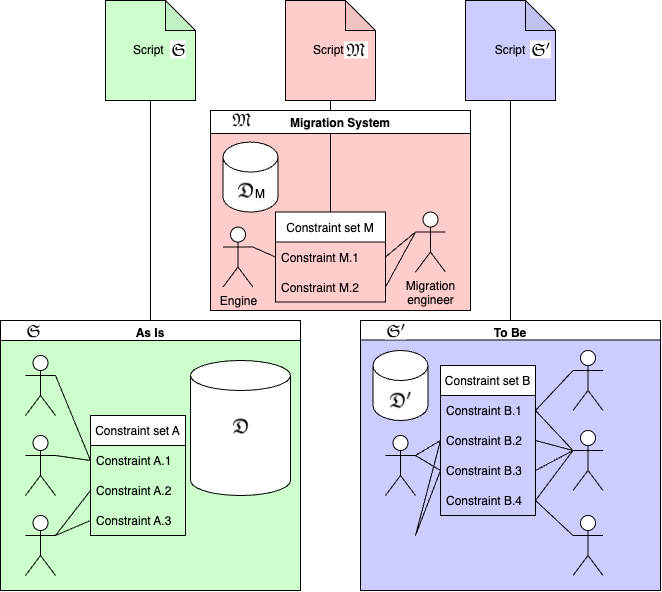
\includegraphics[scale=.45]{Migration.drawio.png}
	\end{center}
\caption{migration}
\label{fig:event flow}
\end{figure}
		
	We use two datasets: $\dataset=\la\atoms,\concepts,\inst,\isa,\rels,\triples\ra$ and $\dataset'=\la\atoms',\concepts',\inst',\isa',\rels',\triples'\ra$.
	Before doing so, let us first define the disjoint union of two information systems.
\begin{definition}[disjoint union of datasets]
	\begin{eqnarray}
		\dataset\sqcup\dataset'&=&\la\atoms\sqcup\atoms',\ \concepts\sqcup\concepts',\ \inst\sqcup\inst',\ \isa\sqcup\isa',\ \rels\sqcup\rels',\ \triples\sqcup\triples'\ra\\
		\atoms\sqcup\atoms'&=&\{(a,0)|\ a\in\atoms\}\ \cup\ \{(a',1)|\ a'\in\atoms'\}\\
		\concepts\sqcup\concepts'&=&\{(c,0)|\ c\in\concepts\}\ \cup\ \{(c',1)|\ c'\in\concepts'\}\\
		\inst\sqcup\inst'&=&\begin{array}[t]{@{}l}
							  \{((a,0),(A,0))|\ (a,A)\in\inst\}\ \cup\\
			                  \{((a',1),(A',1))|\ (a',A')\in\inst'\}
							\end{array}\\
		\isa\sqcup\isa'&=&\begin{array}[t]{@{}l}
							  \{((A,0),(B,0))|\ A\isa B\}\ \cup\\
			                  \{((A',1),(B',1))|\ A'\isa' B'\}
							\end{array}\\
		\rels\sqcup\rels'&=&\{(r,0)|\ r\in\rels\}\ \cup\ \{(r',1)|\ r'\in\rels'\}\\
		\triples\sqcup\triples'&=&\begin{array}[t]{@{}l}
			                        \{\triple{(a,0)}{(r,0)}{(b,0)}|\ \triple{a}{r}{b}\in\triples\}\ \cup\\
			                        \{\triple{(a',1)}{(r',1)}{(b',1)}|\ \triple{a'}{r'}{b'}\in\triples'\}
								   \end{array}
	\end{eqnarray}
\end{definition}
\begin{definition}[$\doteq$]
	\begin{eqnarray}
		\declare{nm}{A}{B}\doteq\declare{nm'}{A'}{B'}&\Leftrightarrow&\id{nm}=\id{nm'}\wedge A=A'\wedge B=B'
	\end{eqnarray}
\end{definition}
\begin{definition}[migration dataset]
	\begin{eqnarray}
		&&\begin{array}[t]{@{}l}
			\{ {\tt ENFORCE\ }\declare{nm'}{A'}{B'}{\tt := }\ident{A'};\declare{nm}{A}{B};\ident{B'}\\
				|\ \begin{array}[t]{@{}l}
					\declare{nm}{A}{B}\in\rels\wedge\declare{nm'}{A'}{B'}\in\rels'\wedge\id{nm}=\id{nm'}\ \wedge\\
					\{\pair{A}{A'},\pair{B}{B'}\}\subseteq\isa\cup\isa'\cup\flip{\isa}\cup\flip{\isa'}\}
				   \end{array}
			  \end{array}\\
			  &\cup&\begin{array}[t]{@{}l}
				\{ {\tt CLASSIFY\ }(C',1){\tt\ IS\ }(C,0)|\ C\in\concepts,C'\in\concepts',C=C'\}\\
			  \end{array}
	\end{eqnarray}
\end{definition}
\begin{definition}[disjoint union of information systems]
	\begin{eqnarray}
		\infsys\sqcup\infsys'&=&\la\roles\sqcup\roles',\rules\sqcup\rules',\maintain\sqcup\maintain',\dataset\sqcup\dataset'\ra\\
		\roles\sqcup\roles'&=&\{(r,0)|\ r\in\roles\}\ \cup\ \{(r',1)|\ r'\in\roles'\}\\
		\rules\sqcup\rules'&=&\{(r,0)|\ r\in\rules\}\ \cup\ \{(r',1)|\ r'\in\rules'\}\\
		\maintain\sqcup\maintain'&=&\begin{array}[t]{@{}l}
							  \{((o,0),(u,0))|\ (o,u)\in\maintain\}\ \cup\\
			                  \{((o',1),(u',1))|\ (o',u')\in\maintain'\}
							\end{array}
	\end{eqnarray}
\end{definition}

\subsection{Changes}
% The purpose of this section is to explain why a dataset is structured the way it is.
	In the migration of a dataset we deal with changes to the elements that are not data:
	$\isa$, $\inst$, $\concepts$, and $\rels$.
	Such changes have further reaching consequences, however.
	Changes to $\isa$, $\inst$, $\concepts$, $\rels$ change the data structure in a dataset.
	We define a \define{migration of a dataset} $\la\atoms,\concepts,\inst,\isa,\rels,\triples\ra$ as a change in which one or more of $\isa$, $\inst$, $\concepts$, or $\rels$ change.
	To satisfy definition~\ref{def:dataset}, $\triples$ and $\atoms$ must change too,
	but the migration should try to preserve the maximal amount of data.

	This paper studies those changes and seeks to preserve the rules in definition~\ref{def:dataset}
	in such a way that large portions of migration can be automated.


\section{Bibliography}
\bibliographystyle{elsarticle-harv}
\bibliography{doc}


\end{document}
